\subsection{2D lid-driven cavity}

\begin{frame}{Stationary and dimensionless Navier-Stokes equations}
  \vspace{-5mm}
	\begin{columns}
		\begin{column}{0.6\textwidth}%
			\begin{align*}
				-\frac{1}{Re} \Delta v + (v \cdot \nabla)v + \nabla p & = 0 \;   & {\rm in}\; \Omega           \\
				{\rm div}(v)                                          & = 0 \;   & {\rm in} \; \Omega          \\
				v                                                     & = v_0 \; & {\rm on} \; \partial \Omega
			\end{align*}
  \vspace{-4mm}
			\begin{itemize}
				\item $v_0=(1,0)$ on the lid and zero everywhere else
        \item $P_1\textrm{-}P_1\textrm{-}Stab$ (Bochev-Dohrmann) \footnotemark{}
				\item Subdomain size: $150\times 150$ elements
				\item Solver absolute and relative tolerances: \num{e-6}
        \item RGDSW coarse space \footnotemark{}
				\item Hybrid-1 variant
			\end{itemize}
		\end{column}
		\begin{column}{0.4\textwidth}
			\begin{figure}
				\centering
				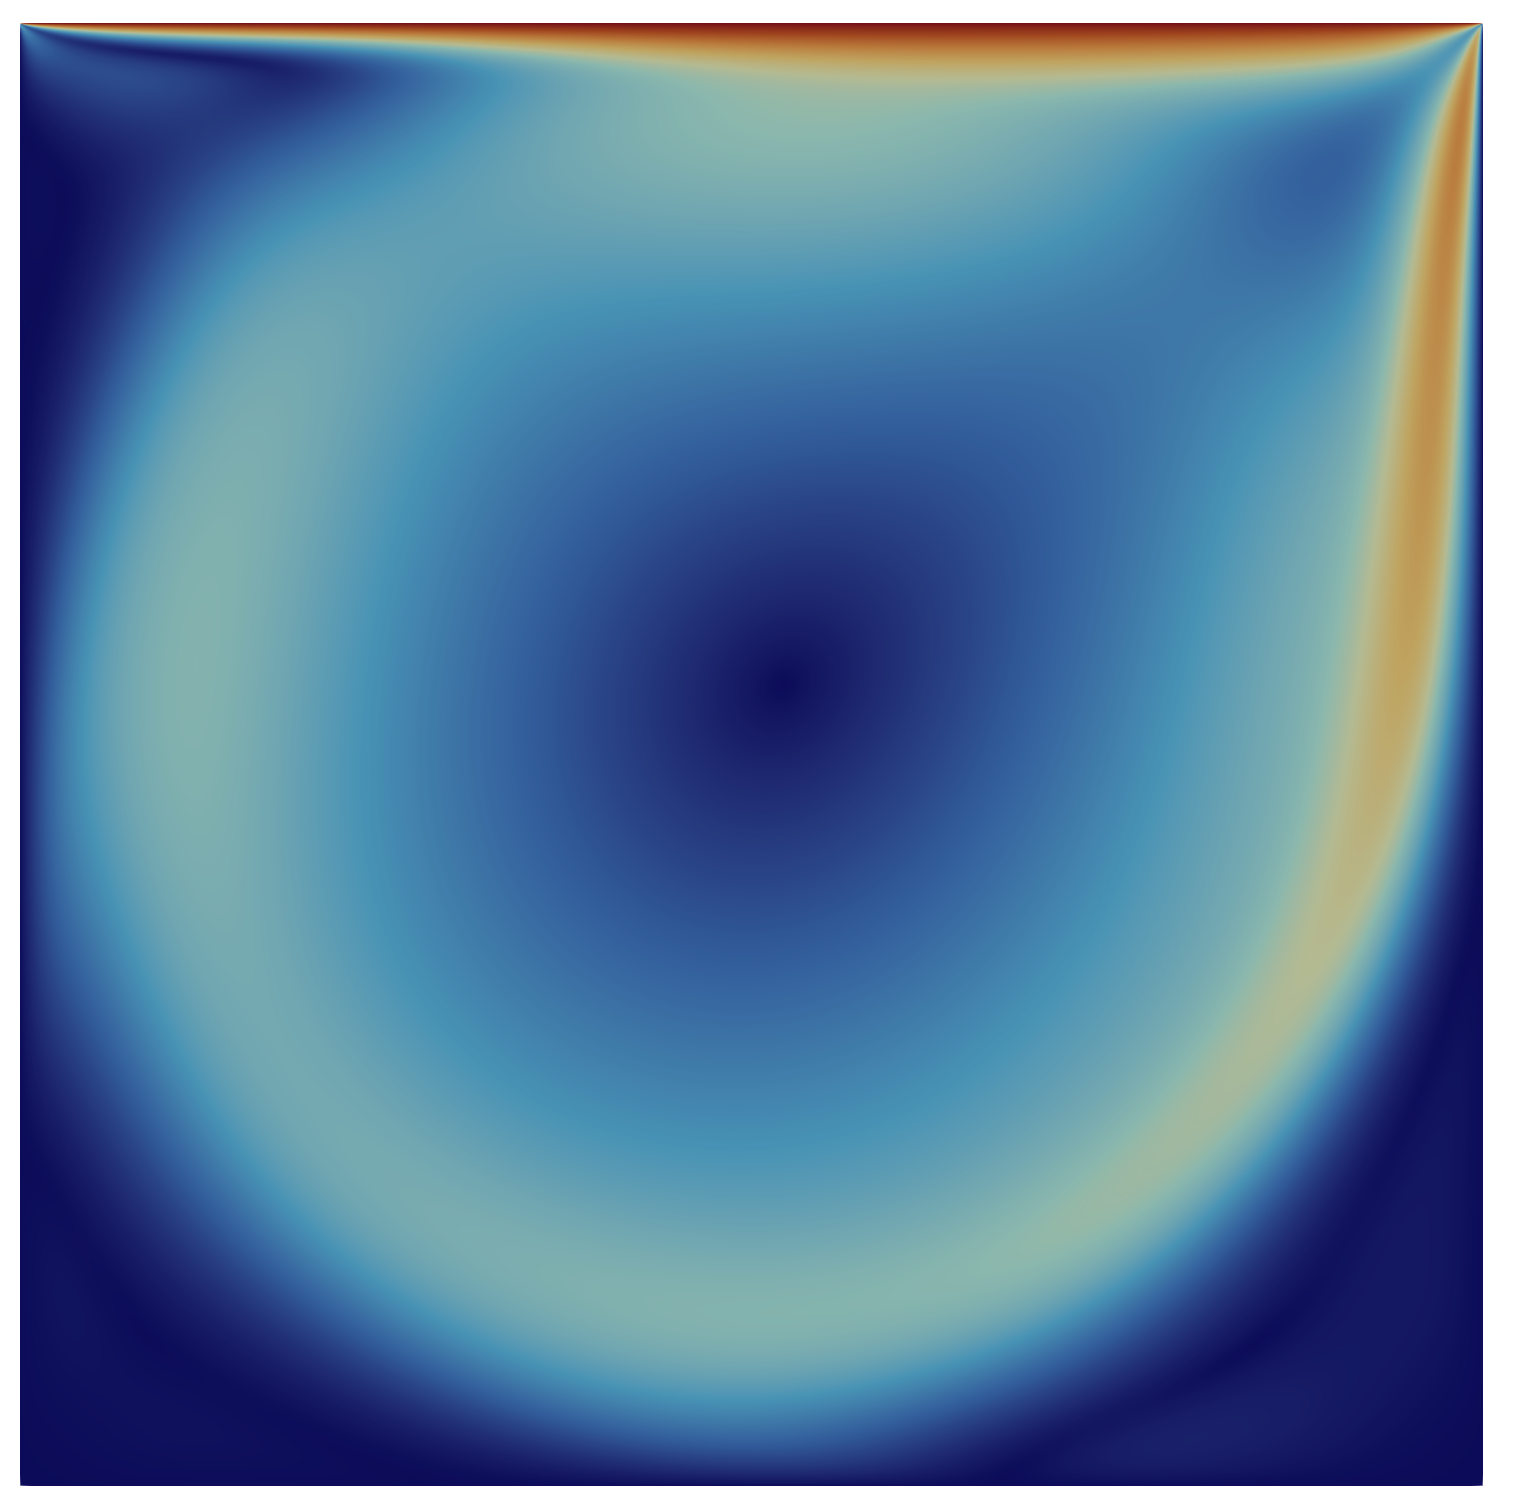
\includegraphics[width=0.7\textwidth]{images/ldc.png}
				\caption{Lid-driven cavity}
			\end{figure}
		\end{column}
	\end{columns}
  \footnotetext[5]{\tiny Dohrmann, Bochev (2004)}
  \footnotetext{\tiny Dohrmann, Widlund (2017)}
\end{frame}

\begin{frame}{Lid-driven cavity: Newton-Krylov-Schwarz vs Hybrid-1}
	\begin{itemize}
		\item $256$ subdomains
	\end{itemize}
	\begin{figure}
		\centering
		\begin{tikzpicture}
    \begin{groupplot}[
        group style={group size=1 by 2, vertical sep=1.cm},
        width=13cm, height=4cm,
        xlabel={Iter.},
        grid=major,
        log basis y=10,
        legend style={at={(1.0,0.9)},anchor=east},
				xmin=0,
				xmax=30,
				ymin=1e-6,
				ymax=1,
        every axis plot/.append style={line width=1pt, mark size=1.5pt, mark=*},
    ]
    \nextgroupplot[
        ylabel={Rel. residual},
        ymode=log,
    ]
    \addplot coordinates {
        (0, 1) (1, 0.00320133) (2, 0.00143493) (3, 0.000610389) 
        (4, 0.000369944) (5, 0.000215426) (6, 1.11767e-05) (7, 4.18693e-08)
    };
    \addlegendentry{Re=500}
    \addplot coordinates {
        (0, 1) (1, 0.00480191) (2, 0.00380737) (3, 0.00297334)
        (4, 0.00272655) (5, 0.00272013) (6, 0.00270843) (7, 0.00268613)
        (8, 0.00267774) (9, 0.00266959) (10, 0.00243689) (11, 0.0024165)
        (12, 0.00223072) (13, 0.00221035) (14, 0.002201) (15, 0.00219758)
        (16, 0.00219347) (17, 0.00219139) (18, 0.00219044) (19, 0.00219027)
        (20, 0.00218816) (21, 0.00218768) (22, 0.0021868) (23, 0.00218531)
        (24, 0.00218251) (25, 0.00217408) (26, 0.00217307) (27, 0.00217296)
        (28, 0.00217293) (29, 0.00217293)
    };
    \addlegendentry{Re=750}
    \addplot coordinates {
        (0, 1) (1, 0.00640242) (2, 0.00404174) (3, 0.00228814)
        (4, 0.00160117) (5, 0.00132757) (6, 0.00119772) (7, 0.00119687)
        (8, 0.00119643) (9, 0.00119643) (10, 0.00119643) (11, 0.00119643)
        (12, 0.00119643) (13, 0.00119643) (14, 0.00119643) (15, 0.00119643)
        (16, 0.00119643) (17, 0.00119643) (18, 0.00119643) (19, 0.00119643)
        (20, 0.00119643) (21, 0.00119643) (22, 0.00119643) (23, 0.00119643)
        (24, 0.00119643) (25, 0.00119643) (26, 0.00119643) (27, 0.00119643)
        (28, 0.00119643) (29, 0.00119643)
    };
    \addlegendentry{Re=1000}


    % Absolute residual plot
    \nextgroupplot[
        ylabel={Rel. residual},
        ymode=log,
    ]
    \addplot coordinates {
        (0, 1) (1, 0.00333167) (2, 0.00171) (3, 0.000567273) (4, 2.88754e-05) (5, 2.1e-6)
    };
    \addlegendentry{$Re=500$}

    \pgfplotsset{cycle list shift=1}
    \addplot coordinates {
        (0, 1) (1, 0.00697345) (2, 0.00505459) (3, 0.00145207) (4, 0.000179099) (5, 4.02319e-05) (6, 1.2e-5)
    };
    \addlegendentry{$Re=1000$}
    \addplot coordinates {
        (0, 1) (1, 0.0230643) (2, 0.0281636) (3, 0.00752757) (4, 0.0038533) (5, 0.000431891) 
        (6, 0.00015685) (7, 0.000106818) (8, 3.3031e-05)
    };
    \addlegendentry{$Re=3000$}
    \addplot coordinates {
        (0, 1) (1, 0.0450654) (2, 0.0419026) (3, 0.0211182) (4, 0.0136736) 
        (5, 0.00420034) (6, 0.00240511) (7, 0.00147275) (8, 0.00133153) 
        (9, 0.00109276) (10, 0.000921041) (11, 0.000763891) (12, 0.000543994) 
        (13, 0.000396203) (14, 0.000265624) (15, 0.00017063) (16, 0.000113675)
    };
    \addlegendentry{$Re=6000$}

    % \addplot coordinates {
    %     (0, 0.0979592) (1, 0.0003136) (2, 0.000140565) (3, 5.97932e-05) 
    %     (4, 3.62394e-05) (5, 2.11029e-05) (6, 1.09486e-06) (7, 4.10148e-09)
    % };
    % \addlegendentry{Re=500}
    % \addplot coordinates {
    %     (0, 0.0653061) (1, 0.000313594) (2, 0.000248645) (3, 0.000194177) 
    %     (4, 0.000178061) (5, 0.000177641) (6, 0.000176877) (7, 0.000175421) 
    %     (8, 0.000174873) (9, 0.000174341) (10, 0.000159144) (11, 0.000157812) 
    %     (12, 0.00014568) (13, 0.00014435) (14, 0.000143739) (15, 0.000143515) 
    %     (16, 0.000143247) (17, 0.000143111) (18, 0.000143049) (19, 0.000143038) 
    %     (20, 0.0001429) (21, 0.000142869) (22, 0.000142811) (23, 0.000142714) 
    %     (24, 0.000142531) (25, 0.000141981) (26, 0.000141915) (27, 0.000141908) 
    %     (28, 0.000141906) (29, 0.000141905)
    % };
    % \addlegendentry{Re=750}
    % \addplot coordinates {
    %     (0, 0.0489796) (1, 0.000313588) (2, 0.000197963) (3, 0.000112072) 
    %     (4, 7.84249e-05) (5, 6.5024e-05) (6, 5.86639e-05) (7, 5.86224e-05) 
    %     (8, 5.86006e-05) (9, 5.86004e-05) (10, 5.86004e-05) (11, 5.86005e-05) 
    %     (12, 5.86004e-05) (13, 5.86004e-05) (14, 5.86004e-05) (15, 5.86004e-05) 
    %     (16, 5.86004e-05) (17, 5.86004e-05) (18, 5.86004e-05) (19, 5.86004e-05) 
    %     (20, 5.86004e-05) (21, 5.86004e-05) (22, 5.86007e-05) (23, 5.86005e-05) 
    %     (24, 5.86005e-05) (25, 5.86005e-05) (26, 5.86005e-05) (27, 5.86005e-05) 
    %     (28, 5.86005e-05) (29, 5.86005e-05)
    % };
    % \addlegendentry{Re=1000}

    % Relative residual plot
    \end{groupplot}
\end{tikzpicture}

		\label{fig:residual-ldc}
	\end{figure}
\end{frame}

\begin{frame}{Lid-driven cavity: nonlinear Schwarz weak scalability}
	\begin{figure}
		\centering
		\begin{tikzpicture}
	\pgfplotsset{
		every axis/.append style={
				ybar stacked,
				width=13cm,
				height=7cm,
				ylabel={Runtime (seconds)},
				xlabel={Num. subdomains},
				symbolic x coords={256, 576, 1024, 2025, 4096, 9216},
				xtick=data,
				enlarge x limits=0.15,
				legend style={at={(1,1)},anchor=north west},
				axis lines*=left, ymajorgrids, yminorgrids,
				ymin=0,
				ymax=500,
				bar width=8pt,
				minor y tick num=1,
				xticklabel style={rotate=0,xshift=0ex,anchor=north},
				cycle list name=Set2-5,
			},
		% Ensures that bars are plotted full
		every axis plot/.append style={
				fill,
			},
	}
  \tikzstyle{mynodestyle} = [rotate=90, anchor=west]

	% Re = 1000
	\begin{axis}[bar shift=-11pt, hide axis]
		% Another option for relative node placement
		% \node [left=11pt of 256.base, anchor=base] {test}; % Custom number above bar for 256
		\node[mynodestyle] (one) at ([xshift=-11pt]axis cs:256,183) {$720$ $(6)$};
		\node[mynodestyle] at ([xshift=-11pt]axis cs:576,160) {$520$ $(5)$};
		\node[mynodestyle] at ([xshift=-11pt]axis cs:1024,126){$350$ $(4)$};
		\node[mynodestyle] at ([xshift=-11pt]axis cs:2025,129){$310$ $(4)$};
		\node[mynodestyle] at ([xshift=-11pt]axis cs:4096,130){$250$ $(4)$};
		\node[mynodestyle] at ([xshift=-11pt]axis cs:9216,220){$290$ $(5)$};
		\node (oneRe) at ([xshift=-11pt]axis cs:256,15) {$1$};

		\addplot coordinates {(256,33) (576,29) (1024,25) (2025,25) (4096,25) (9216,30)};
		\addplot+ coordinates {(256,27) (576,26) (1024,26) (2025,29) (4096,31) (9216,55.8)};
		\addplot+ coordinates {(256,71) (576,56) (1024,35) (2025,33) (4096,29.5) (9216,83)};
		\addplot+ coordinates {(256,51.7) (576,47.3) (1024,40) (2025,42) (4096,44.5) (9216,55.2)};

	\end{axis}

	% Re = 2000
	\begin{axis}[bar shift=0pt, hide axis]
		\node[mynodestyle](256) at (axis cs:256,239) {$1000$ $(7)$};
		\node[mynodestyle](576) at (axis cs:576,223) {$820$ $(6)$};
		\node[mynodestyle](1024) at (axis cs:1024,178) {$610$ $(5)$};
		\node[mynodestyle](2025) at (axis cs:2025,140) {$390$ $(4)$};
		\node[mynodestyle](4096) at (axis cs:4096,138) {$300$ $(4)$};
		\node[mynodestyle](9216) at (axis cs:9216,240) {$300$ $(5)$};
		\node at (axis cs:256,15) {$2$};

		\addplot+ coordinates {(256,44) (576,40) (1024,32) (2025,26) (4096,26) (9216,32)};
		\addplot+ coordinates {(256,32) (576,32) (1024,30) (2025,29) (4096,33) (9216,72)};
		\addplot+ coordinates {(256,104) (576,95) (1024,39) (2025,45) (4096,36) (9216,86)};
		\addplot+ coordinates {(256,59) (576,56) (1024,77) (2025,40) (4096,43) (9216,56)};
	\end{axis}

	% Re = 4000

	\begin{axis}[bar shift=11pt]
		\node (three)[rotate=90,anchor=west]at([xshift=11pt]axis cs:256,345) {$1500$ $(9)$};
    \node [mynodestyle] at([xshift=11pt]axis cs:576,400) {$1700$ $(10)$};
		\node [mynodestyle]at([xshift=11pt]axis cs:1024,326) {$1200$ $(8)$};
		\node [mynodestyle]at([xshift=11pt]axis cs:2025,246) {$830$ $(6)$};
		\node [mynodestyle]at([xshift=11pt]axis cs:4096,201) {$580$ $(5)$};
		\node [mynodestyle]at([xshift=11pt]axis cs:9216,285) {$430$ $(5)$};
		\node at ([xshift=11pt]axis cs:256,15) {$4$};

		\addplot+ coordinates {(256,61) (576,66) (1024,53) (2025,42) (4096,34) (9216,33.7)};
		\addplot+ coordinates {(256,42) (576,52) (1024,49) (2025,44) (4096,43) (9216,75)};
		\addplot+ coordinates {(256,167) (576,202) (1024,150) (2025,101) (4096,72) (9216,125)};
		\addplot+ coordinates {(256,75) (576,88) (1024,74) (2025,59) (4096,52) (9216,55.8)};

    \node[anchor=south,text width=1.6cm] (gmres) at (axis cs:256,440){GMRES its. (Newton its.)};

		\legend{
			Inner solve,
			Coarse solve,
			GMRES,
			Other
		}

	\end{axis}

	\node[rotate=0, text width=1.8cm] (Re) at ([yshift=-110,xshift=-18]256){Re ($\times 10^{3}$)};

	\draw [thin] (gmres) --  (256);
	\draw [thin] (gmres) --  (one);
	\draw [thin] (gmres) --  (three);

	\draw [thin] (Re) --  (oneRe);

\end{tikzpicture}

		\label{fig:weak-scalability-nls}
	\end{figure}
\end{frame}

\begin{frame}{Lid-driven cavity: nonlinear Schwarz weak scalability}
	\begin{figure}
		\centering
		\begin{tikzpicture}
	\pgfplotsset{
		every axis/.append style={
      ybar stacked,
      width=13cm,
      height=7cm,
      ylabel={Avg. runtime per iter. (seconds)},
      xlabel={Num. subdomains},
      symbolic x coords={256, 576, 1024, 2025, 4096, 9216},
      xtick=data,
      enlarge x limits=0.15,
      legend style={at={(0,1)},anchor=north west},
      axis lines*=left, ymajorgrids,
      ymin=0,
      ymax=60,
      bar width=8pt,
      nodes near coords,
      nodes near coords style={rotate=90},
      minor y tick num=1,
      xticklabel style={rotate=0,xshift=0ex,anchor=north},
      cycle list name=Set2-5,
    },
		% Ensures that bars are plotted full
		every axis plot/.append style={
      fill,
			% fill opacity=0.5,
      every node/.append style={
        text=black,
      },
    },
	}
% Re = 1000
	\begin{axis}[bar shift=-11pt, hide axis]
    \addplot+ coordinates {(256,5.5) (576,5.8) (1024,6.3) (2025,6.3) (4096,6.3)   (9216,6)};   
    \addplot+ coordinates {(256,4.5) (576,5.2) (1024,6.5) (2025,7.3) (4096,7.8)   (9216,11.2)}; 
    \addplot+ coordinates {(256,11.8) (576,11.2) (1024,8.8) (2025,8.3) (4096,7.4) (9216,16.6)};   
    \addplot+ coordinates {(256,8.6) (576,9.5) (1024,10.0) (2025,10.5) (4096,11.1) (9216,11)}; 
	\end{axis}

% Re = 2000
	\begin{axis}[bar shift=0pt, hide axis]
    \addplot+ coordinates {(256,6.3) (576,6.7) (1024,6.4) (2025,6.5) (4096,6.5)   (9216,6.4)};  
    \addplot+ coordinates {(256,4.6) (576,5.3) (1024,6.0) (2025,7.3) (4096,8.3)   (9216,14.4)};  
    \addplot+ coordinates {(256,14.9) (576,15.8) (1024,7.8) (2025,11.3) (4096,9.0) (9216,17.2)}; 
    \addplot+ coordinates {(256,8.4) (576,9.3) (1024,15.4) (2025,10.0) (4096,10.8)(9216,11.2)};  
	\end{axis}

% Re = 4000
	\begin{axis}[bar shift=11pt]
    \addplot+ coordinates {(256,6.8) (576,6.6) (1024,6.6) (2025,7.0) (4096,6.8)      (9216,6.7)}; 
    \addplot+ coordinates {(256,4.7) (576,5.2) (1024,6.1) (2025,7.3) (4096,8.6)      (9216,15)};   
    \addplot+ coordinates {(256,18.6) (576,20.2) (1024,18.8) (2025,16.8) (4096,14.4) (9216,25)};  
    \addplot+ coordinates {(256,8.3) (576,8.8) (1024,9.3) (2025,9.8) (4096,10.4)     (9216,11.2)}; 

		\legend{
			Inner solve,
			Coarse solve,
			GMRES,
			Other
		}
  \end{axis}
\end{tikzpicture}

		\label{fig:weak-scalability-per-iter-nls}
	\end{figure}
\end{frame}

\begin{frame}{LDC coarse basis functions}
	\begin{figure}
		\centering
		\begin{subfigure}{0.5\textwidth}
			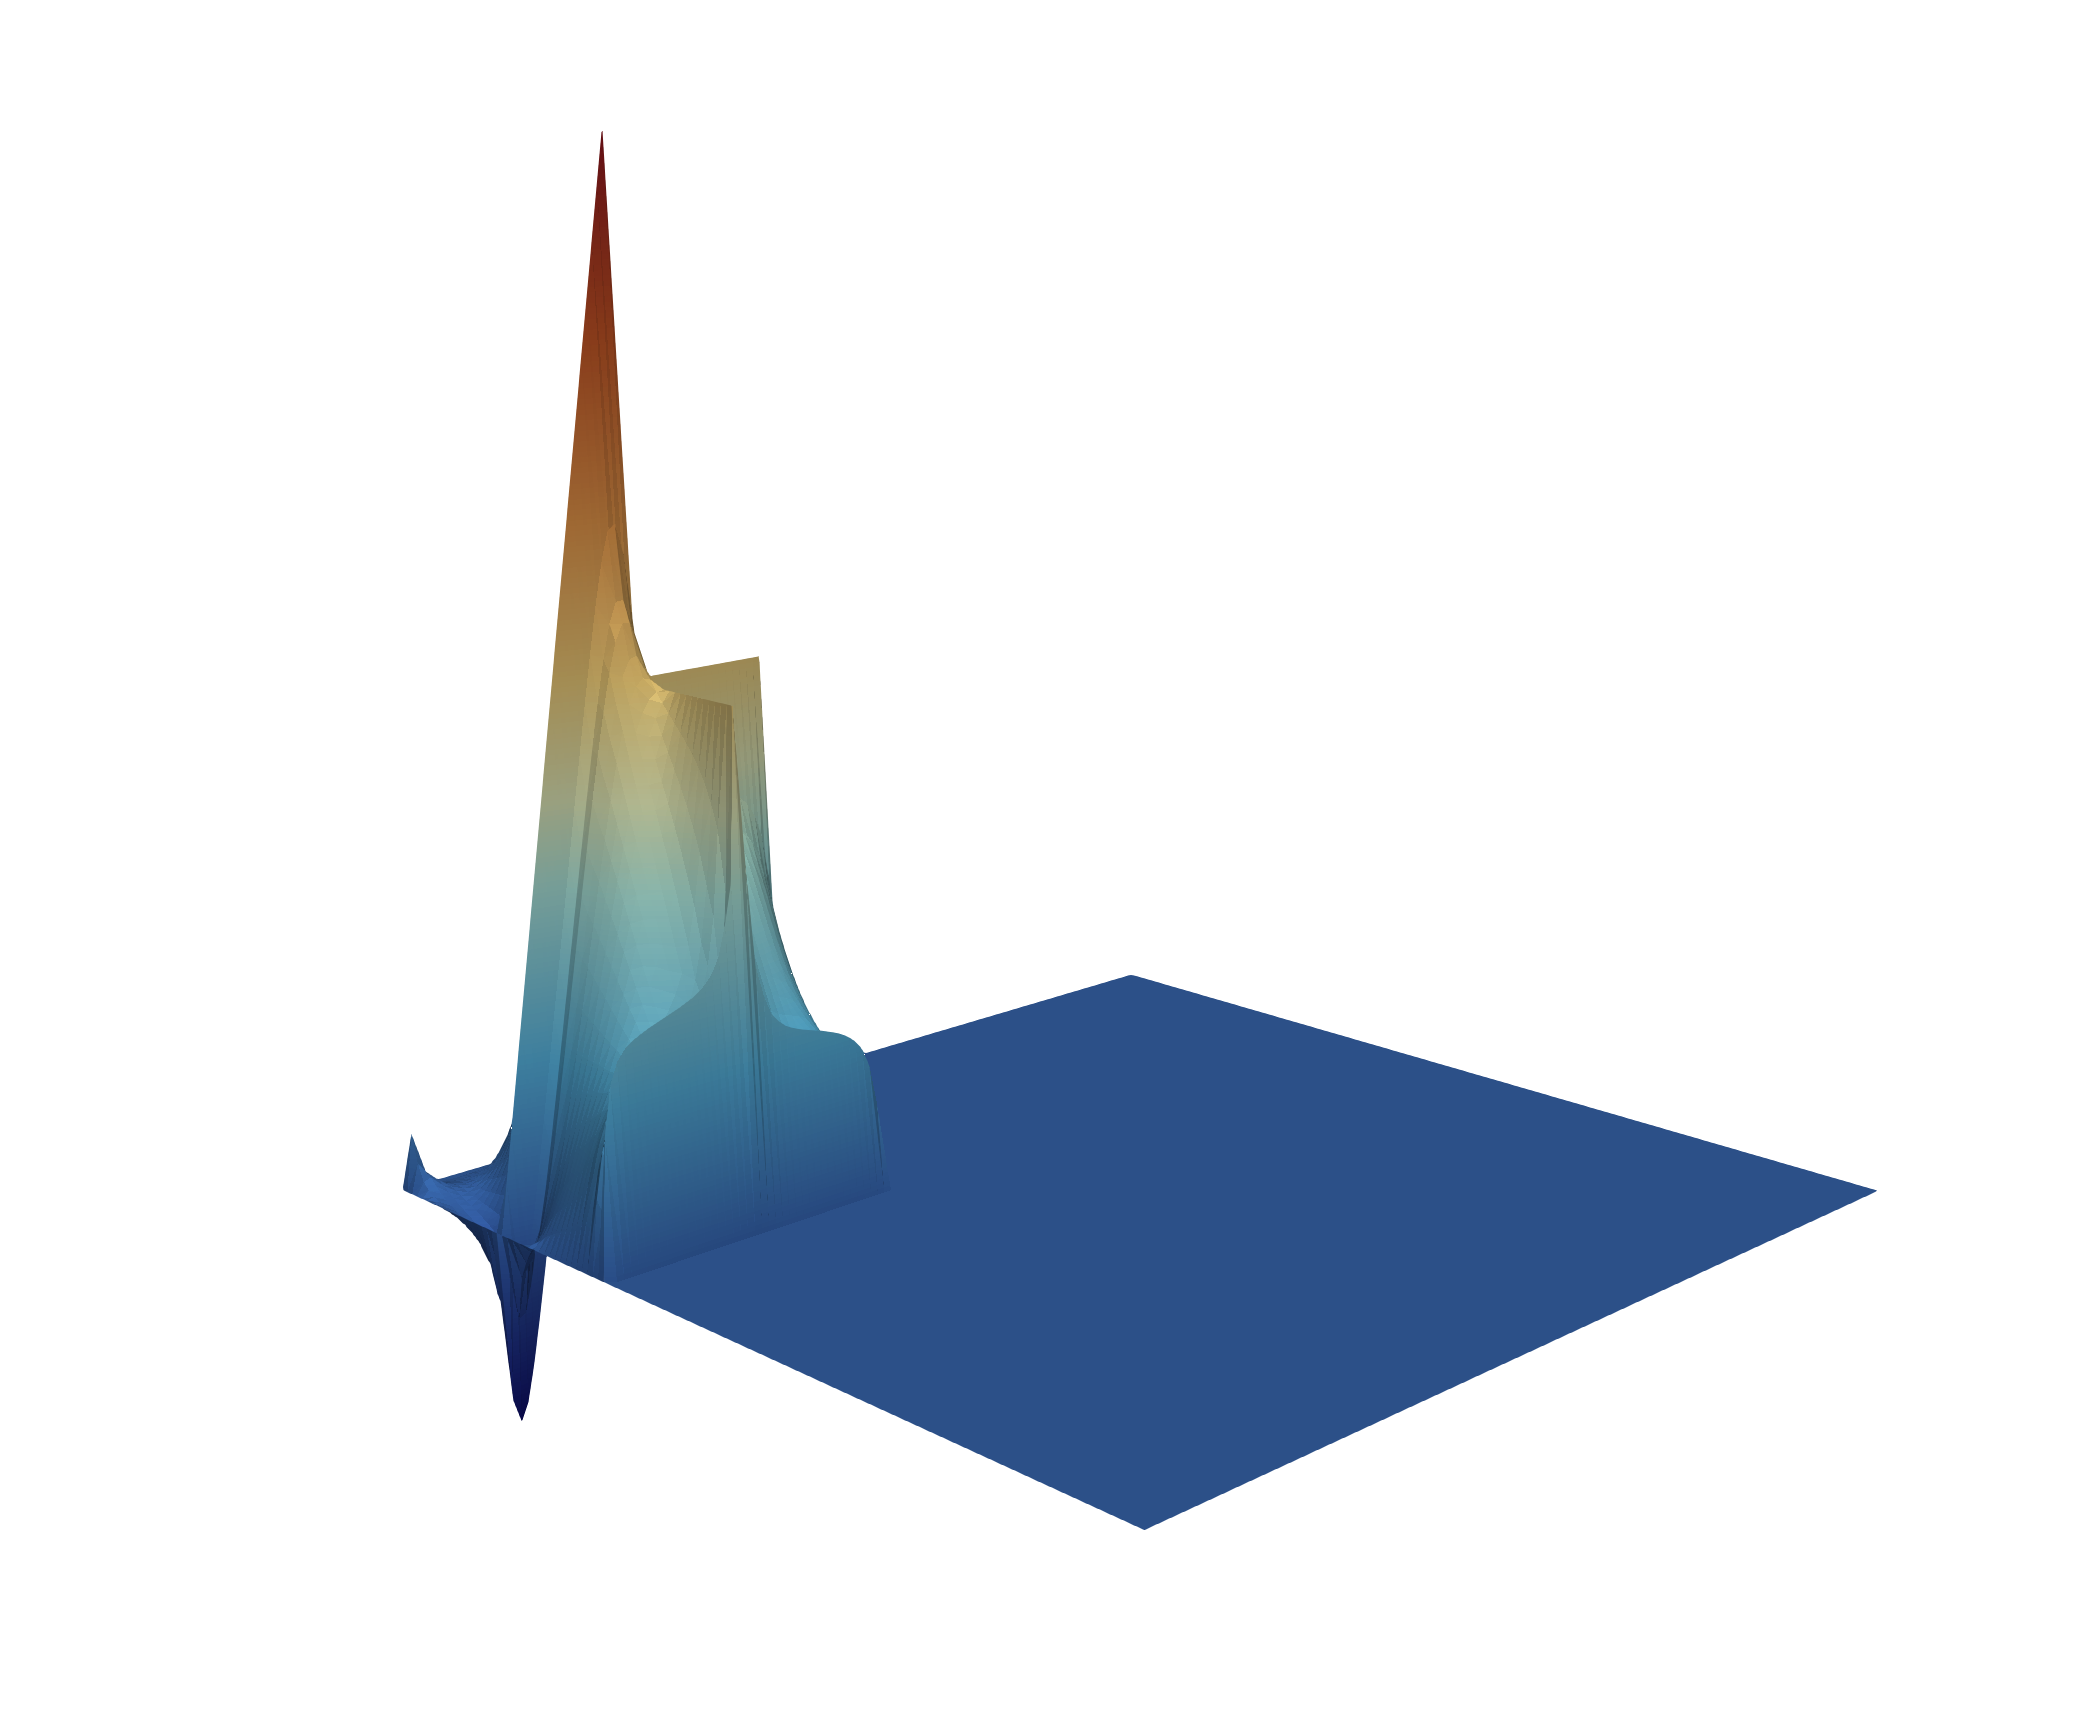
\includegraphics[width=\textwidth]{images/RGDSW-x}
			\caption{RGDSW $x$ component.}
		\end{subfigure}%
		\begin{subfigure}{0.5\textwidth}
			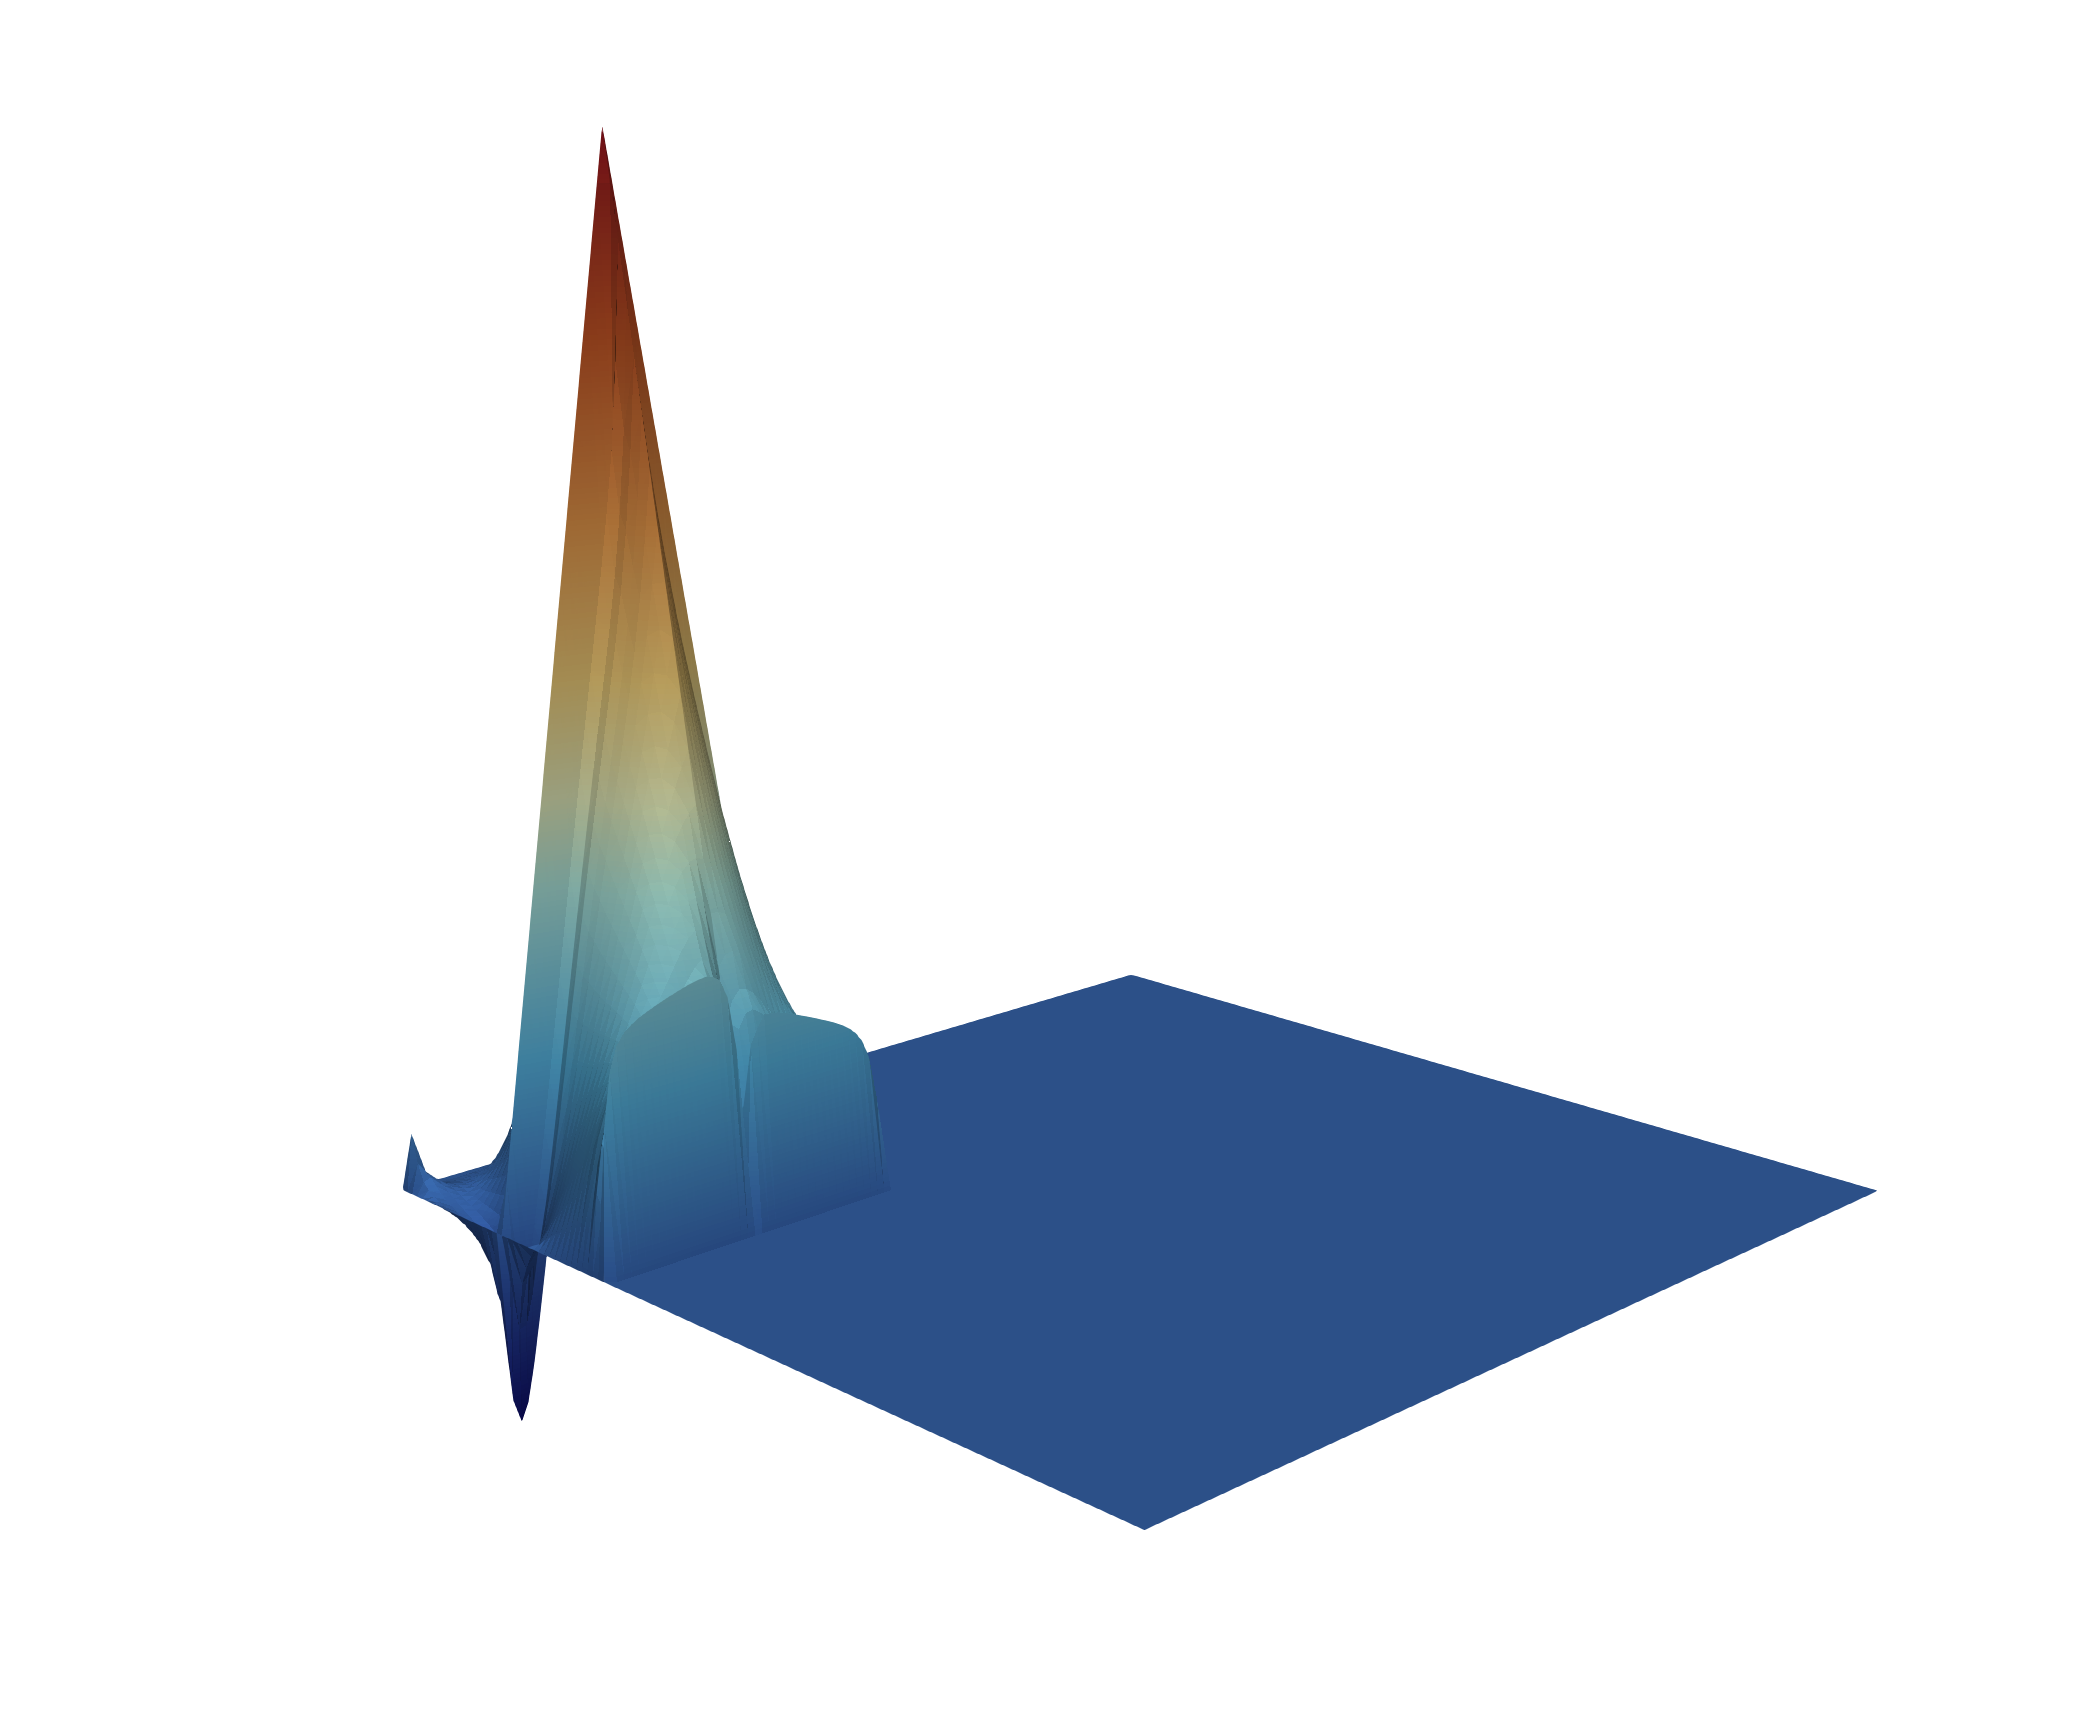
\includegraphics[width=\textwidth]{images/MsFEM-x}
			\caption{MsFEM $x$ component.}
		\end{subfigure}
		\caption{Components of $x$ velocity coarse basis function.}
	\end{figure}
\end{frame}

\begin{frame}{MsFEM vs. RGDSW}
	% Mention that: 
	%   - Re has no effect 
	%   - MsFEM was faster for Re=1000 but maybe RGDSW can be sped up with proper tuning
	%   - These results were generated with higher GMRES tollerance which increases GMRES count and runtime without a positive effect
	\begin{itemize}
		\item $256$ subdomains
	\end{itemize}
	\begin{figure}
		\centering
		\begin{tikzpicture}
	\pgfplotsset{
		every axis/.append style={
				ybar stacked,
				width=13cm,
				height=7cm,
				ylabel={Runtime (seconds)},
				xlabel={$Re$},
				symbolic x coords={1000,2000,2750,4000,5000,6000,7000},
				xtick=data,
				enlarge x limits=0.15,
				legend style={at={(0.9,1)},anchor=north west},
				axis lines*=left, ymajorgrids, yminorgrids,
				ymin=0,
				ymax=1800,
				bar width=12pt,
				minor y tick num=1,
				xticklabel style={rotate=0,xshift=0ex,anchor=north},
				cycle list name=Set2-5,
			},
		% Ensures that bars are plotted full
		every axis plot/.append style={
				fill,
			},
	}
	% RGDSW
	\begin{axis}[bar shift=-8pt, hide axis]
		\node [rotate=90](rgdsw) at ([xshift=-8pt]axis cs:1000,150) {RGDSW};
		% Inner solve
		\addplot coordinates {(1000,33) (2000,45) (2750,54) (4000,61) (5000,74) (6000,104)      };
		% Coarse solve
		\addplot coordinates {(1000,27) (2000,32) (2750,40) (4000,42) (5000,51) (6000,69)       };
		% GMRES
		\addplot coordinates {(1000,222) (2000,340) (2750,430) (4000,559) (5000,734) (6000,1142)};
		% Other
		\addplot coordinates {(1000,52) (2000,59) (2750,67) (4000,76) (5000,90) (6000,130)      };

    \node [rotate=90,anchor=west](1000) at ([xshift=-8pt]axis cs:1000,334) {$1700$ $(6)$};
		\node [rotate=90,anchor=west](2000) at ([xshift=-8pt]axis cs:2000,476) {$2400$ $(7)$};
		\node [rotate=90,anchor=west](2750) at ([xshift=-8pt]axis cs:2750,591) {$2900$ $(8)$};
		\node [rotate=90,anchor=west](4000) at ([xshift=-8pt]axis cs:4000,738) {$3600$ $(9)$};
		\node [rotate=90,anchor=west](5000) at ([xshift=-8pt]axis cs:5000,949) {$4600$ $(11)$};
		\node [rotate=90,anchor=west](6000) at ([xshift=-8pt]axis cs:6000,1445) {$7000$ $(16)$};
		% \node [rotate=90,anchor=west](7000) at ([xshift=-8pt]axis cs:7000,2818) {$14000$ $(30)$};

	\end{axis}

	%  (7000,202)
	%  (7000,139)
	% (7000,2243)
	%  (7000,234)	

	\begin{axis}[bar shift=8pt]
		\node [rotate=90](msfem) at ([xshift=8pt]axis cs:1000,140) {MsFEM};
		% Inner solve
		\addplot coordinates {(1000,34) (2000,58) (2750,74) (4000,0) (5000,0) (6000,0) };
		% Coarse solve
		\addplot coordinates {(1000,39) (2000,59) (2750,63) (4000,0) (5000,0) (6000,0) };
		% GMRES
		\addplot coordinates {(1000,174) (2000,345) (2750,468) (4000,0) (5000,0) (6000,0) };
		% Other
		\addplot coordinates {(1000,53) (2000,75) (2750,91) (4000,0) (5000,0) (6000,0) };

		\legend{
			Inner solve,
			Coarse solve,
			GMRES,
			Other
		}
		\node[rotate=90,anchor=west](one) at ([xshift=8pt]axis cs:1000,300) {$1400$ $(6)$};
		\node[rotate=90,anchor=west] at ([xshift=8pt]axis cs:2000,537) {$2600$ $(9)$};
		\node[rotate=90,anchor=west] at ([xshift=8pt]axis cs:2750,696) {$3400$ $(11)$};

    \node at ([xshift=8pt]axis cs:4000,40) {\scriptsize\color{red}\ding{55}};
		\node at ([xshift=8pt]axis cs:5000,40) {\scriptsize\color{red}\ding{55}};
    \node at ([xshift=8pt]axis cs:6000,40) {\scriptsize\color{red}\ding{55}};


	\end{axis}

	\node[rotate=0, text width=1.6cm] (gmres) at ([xshift=8,yshift=50]1000){GMRES its. (Newton its.)};
	% \node[rotate=0, text width=1.8cm] (coarsespace) at ([yshift=-60,xshift=-10]1000){Coarse space};

	\draw [thin] (gmres) --  (1000);
	\draw [thin] (gmres) --  (one);

	% \draw [thin] (coarsespace) --  (rgdsw);
	% \draw [thin] (coarsespace) --  (msfem);

\end{tikzpicture}

		\label{fig:msfem-vs-rgdsw}
	\end{figure}
\end{frame}

\begin{frame}{Summary lid-driven cavity}
	\begin{itemize}
    \item H1 more robust than NKS against nonlinearity
    \item It's weak scaling is excellent up to $4096$ subdomains\\then coarse solve time increases % (larger coarse space improves nonlinear preconditioning)
		\item It's difficult to tune e.g. what makes a good coarse space?%: many parameters that have a potentialy significant impact on performance
	\end{itemize}

	\begin{figure}
		\includegraphics[width=0.55\textwidth]{images/nls.png}
	\end{figure}
	% Bottom line: very sensitive to proper tuning, The coarse space does not encode the Re somehow but it's discretisation properties are critical.
\end{frame}


